\chapter{Aufbau der Fallstudie}
\label{sec:fallstudie}

Im Rahmen dieser Masterarbeit soll nun mithilfe von Hadoop und der Selfbalancing"=Komponente eine Fallstudie durchgeführt werden, durch die ermittelt wird, unter welchen Umständen eine Testautoamtisierung möglich ist.
Dazu werden zunächst Anforderungen an das Hadoop"=System selbst gestellt, die es im Rahmen dieser Tests erfüllen soll.
Neben diesen funktionalen Anforderungen werden aber auch Anforderungen an das Testsystem selbst gestellt, die durch die Tests selbst erfüllt sein sollen.
Zur Realisierung dieser Tests wird mithilfe des \ac{ss}"=Frameworks ein vereinfachtes Modell entwickelt und dieses mit einem realen Cluster verbunden.
Um das reale Cluster auszuführen, wird eine für diese Fallstudie angepasste Version der von \citeauthor{zhang2016} entwickelten Plattform Hadoop"=Benchmark genutzt.

Teile der Beiträge und Inhalte dieses Kapitels wurden bereits im Rahmen der Publikation \cite{Eberhardinger2018} publiziert.

\section{Anforderungen an das Cluster und Testsystem}
\label{sec:requirements}

Zur Überprüfung des Clusters und des Testssystems selbst werden hierfür jeweils mehrere Anforderungen gestellt.
Unterschieden wird hierbei zwischen funktionalen Anforderungen an das \gls{SuT} und Anforderungen an das Testsystem.
Während die funktionalen Anforderungen ausschließlich vom Hadoop"=Cluster als \gls{SuT} erfüllt werden müssen, müssen die Test"=Anforderungen vom gesamten Testsystem erfüllt werden.

Mithilfe der im Folgenden definierten Anforderungen soll bereits automatisiert geprüft werden, inwieweit eine Testautomatisierung möglich ist.
Hierfür werden die Anforderungen, sofern möglich, in Form von Constraints ebenfalls im Modell implementiert und während der Ausführung durch das Oracle validiert.

\subsection{Funktionale Anforderungen an das Cluster}
\label{subsec:functionalRequirements}

Obwohl in dieser Masterarbeit der Fokus auf Testautomatisierung und Validieren eines Testsystems liegt, müssen auch die funktionalen Anforderungen an das \gls{SuT}, also das Hadoop"=Cluster selbst, berücksichtigt werden.
Da im Rahmen der Publikation \cite{Eberhardinger2018} ebenfalls der in \cref{sec:clusterSetup} beschriebene, und in dieser Fallstudie genutzte Versuchsaufbau genutzt wurde, wurden im Rahmen dieser Fallstudie auch funktionale Anforderungen an das Cluster selbst durch das Oracle geprüft.
Dies betrifft konkret folgende Anforderungen an das \gls{SuT} \cite{Eberhardinger2018}:

\begin{enumerate}
    \item Ein Task wird vollständig ausgeführt, sofern er nicht abgebrochen wird
    \item Kein Task oder Anwendung wird an inaktive, defekte oder nicht verbundene Nodes gesendet
    \item Die Konfiguration wird aktualisiert, sobald eine entsprechende Regel erfüllt ist
    \item Defekte oder Verbindungsabbrüche werden erkannt
\end{enumerate}

\subsection{Anforderungen an das Testsystem}
\label{subsec:testRequirements}

Neben den funktionalen Anforderungen, gibt es weitere Anforderungen an das gesamte Testsystem.
Diese Anforderungen betreffen das Hadoop"=Cluster, die Selfbalancing"=Komponente, das entwickelte \gls{ss}"=Modell sowie den Treiber zur Kommunikation zwischen Modell und Cluster.
Konkret sind dies folgende Anforderungen an das Testsystem:

\begin{enumerate}
    \item Der \gls{MARP}"=Wert ändert sich, basierend auf den derzeit ausgeführten Anwendungen
    \item Der jeweils aktuelle Status des Clusters wird erkannt und im Modell gespeichert
    \item Defekte Nodes und Verbindungsabbrüche werden erkannt
    \item Im Modell implementierte Komponentenfehler werden im realen Cluster injiziert und repariert
    \item Wenn alle Nodes defekt sind, wird erkannt, dass sich das Cluster nicht mehr rekonfigurieren kann
    \item Ein Test kann vollautomatisch ausgeführt werden
    \item Das Cluster kann ohne Auswirkungen auf seine Funktionsweise auf einem oder mehreren Hosts ausgeführt werden
    \item Es können mehrere Benchmark"=Anwendungen gleichzeitig gestartet und ausgeführt werden
    \item Tests und Testfälle können zeitlich unabhängig und mehrmals ausgeführt werden
\end{enumerate}

Die funktionalen Anforderungen dienen zudem ebenfalls als Anforderungen an das Testsystem und erweitern somit die hier genannten Anforderungen.

Eine Besonderheit bildet die fünfte Anforderung, wonach erkannt werden muss, dass im Cluster keine weitere Rekonfiguration möglich ist.
Wird diese Anforderung verletzt, soll der ausgeführte Test abgebrochen werden, während bei den anderen, auch den funktionalen, Anforderungen dies nur durch das Oracle vermerkt, die Ausführung aber nicht weiter beeinträchtigt werden soll.


\section{Anforderungen an das Testsystem}
\label{sec:evaluationPlan}

Um das Testsystem zu validieren, wurde zunächst ein Evaluationsplan aufgestellt.
In diesem ist festgehalten, was getestet wird, wie die Testfälle aussehen und wie die bei der Ausführung gewonnen Daten organisiert werden.

\subsection{Behauptungen und Variablen}
\label{sec:predictions}

% Was für Behauptungen wurden aufgestellt
\begin{enumerate}
    \setcounter{enumi}{4}
    \item Der jeweils aktuelle Status des Clusters wird erkannt und im Modell gespeichert
    \item Defekte Nodes und Verbindungsabbrüche werden erkannt
    \item Im Modell implementierte Komponentenfehler werden im realen Cluster injiziert und repariert
    \item Wenn alle Nodes defekt sind, wird erkannt, dass sich das Cluster nicht mehr rekonfigurieren kann
    \item Ein Test kann vollautomatisch ausgeführt werden
    \item Das Cluster kann ohne Auswirkungen auf die Funktionsweise auf einem oder beiden Hosts ausgeführt werden
    \item Es können mehrere Benchmark"=Anwendungen gleichzeitig gestartet und ausgeführt werden
    \item Ein Testfall kann zeitlich unabhängig und mehrmals ausgeführt werden
\end{enumerate}

% Was für Variablen wurden dadurch ermittelt

\subsection{Generierung der Testfälle}
\label{sec:testcaseGeneration}

Die Generierung der Testfälle hängt von mehreren Faktoren ab.
Zum einen ist ein Testfall abhängig von der Größe des Clusters, also ob das Cluster auf einem oder beiden Hosts ausgeführt wird und aus wie vielen Nodes das Cluster besteht.
Relevant zur Unterscheidung von Testfällen sind aber auch die ausgeführten Anwendungen.
Da die Auswahl der ausgeführten Anwendungen nicht manuell bestimmt werden soll, wird hierfür ein Transitionssystem verwendet.
Mithilfe dieses Transitionssystems, in dem die Wahrscheinlichkeiten von Wechsel zwischen zwei Anwendungen definiert sind, soll während der Ausführung eines Testfalls zufällig eine nachfolgende Anwendung ausgewählt werden.
Da zum Testen des Clusters der \ac{ss}"=Simulator eingesetzt wird, hängt die Anzahl der Anwendungen primär von der Anzahl der ausgeführten Simulations"=Schritte ab.
Ein weiterer Faktor zur Anzahl der Anwendungen ist die Anzahl an simulierten Clients, da auch getestet werden soll, wie sich das Cluster bei der Ausführung von mehreren parallel gestarteten Anwendungen verhält.
Die zu injizierenden Komponentenfehler, mit denen defekte Nodes und Verbindungsausfälle simuliert werden, werden ebenfalls zufallsbasiert ausgewählt.
Dies gilt auch für das Deaktivieren der Komponentenfehlern.

Die Auswahl der nachfolgenden Anwendungen und die Entscheidung über die Aktivierung und Deaktivierung der Komponentenfehlern wird daher mithilfe eines Zufallsgenerators realisiert.
Hierbei soll jedoch kein echter Zufallsgenerator zum Einsatz kommen, sondern ein Pseudo"=Zufallsgenerator.
Da ein Pseudo"=Zufallsgenerator seine Werte mithilfe eines Start"=\emph{Seeds} auswählt, besteht somit die Möglichkeit durch die Verwendung eines bestimmten Seeds, einen Testfall jederzeit wiederholen zu können.
Zur Auswahl der ersten Testfälle werden daher zeitbasierte Seeds verwendet.
Diese Seeds werden bei der Ausführung notiert und für andere Testfälle verwendet, bei denen andere Punkte der Konfiguration wie \zB die Größe des Clusters, abgeändert werden.
Dadurch ist es möglich, die Auswirkungen einzelner Parameter zu testen und zu evaluieren.
\todo{Wo wird Seed wie genutzt? am besten in implementierung davon!}

\subsection{Organisation und Ausgabe der Daten}
\label{sec:dataOrganisation}

Damit die bei der Ausführung gewonnenen Daten auch zur Evaluation genutzt werden können, wurde hierzu festgelegt, welche Daten während der Ausführung ausgegeben werden.
Alle relevante Daten werden hierzu während der Ausführung der Testfälle in einer Log"=Datei gespeichert.
Zur Unterscheidung von einzelnen Ausführungen werden die Daten klar strukturiert.
Neben den im folgenden beschriebenen Daten werden zudem alle Ein- und Ausgabedaten der SSH"=Verbindungen zwischen \ac{ss} und dem Cluster (vgl. \autoref{sec:aufbauCluster}) in einem eigenen Log gespeichert.

Beim Start der Simulation werden zunächst einige generelle Daten ausgegeben:

\begin{itemize}
    \item Basis"=Seed für die Zufallsgeneratoren
    \item Mindestdauer für einen Simulations"=Schritt
    \item Anzahl der ausgeführten Simulations"=Schritte
    \item Wahrscheinlichkeiten für Aktivierung und Deaktivierung der Komponentenfehler
    \item Angabe, ob vorab generierte Eingabedaten genutzt werden oder diese während der Ausführung eines Testfalls generiert werden
    \item Anzahl genutzter Hosts und Nodes
    \item Pfade verwendeter Scripte auf den Hosts (vgl. \autoref{sec:aufbauCluster})
    \item Bei der Nutzung der REST"=API verwendete URL des Controllers
    \item Auszuführende Benchmarks    
\end{itemize}

Die Ausgabe der Daten der YARN"=Komponenten wird bei jedem Simulations"=Schritt durchgeführt, damit das Verhalten des Clusters berücksichtigt werden kann.
Ausgegeben werde hierbei:

\begin{itemize}
    \item Für jeden Node:
    \begin{itemize}
        \item ID bzw. Name des Nodes
        \item Aktueller Status
        \item Informationen zur Fehleraktivierung
        \item Anzahl ausgeführter Container auf dem Node
        \item Angaben zur Speicherauslastung
        \item Angaben zur CPU"=Auslastung
    \end{itemize}
    
    \item Für jeden Client:
    \begin{itemize}
        \item ID bzw. Name des Clints
        \item Aktuell ausgeführter Benchmark
        \item ID der aktuell ausgeführten Anwendung auf dem Cluster
    \end{itemize}

    \item Für jede Anwendung:
    \begin{itemize}
        \item ID der Anwendung
        \item Bezeichnung der Anwendung
        \item Aktueller und finaler Status der Anwendung
        \item ID bzw. Name des Nodes, auf dem der \ac{AppMstr} ausgeführt wird
    \end{itemize}

    \item Für jeden Attempt:
    \begin{itemize}
        \item ID des Attempts
        \item Aktueller Status des Attempts
        \item ID des \ac{AppMstr}"=Containers
        \item ID bzw. Name des Nodes, auf dem der \ac{AppMstr} ausgeführt wird
    \end{itemize}

    \item Für jeden Container:
    \begin{itemize}
        \item ID des Containers
        \item ID bzw. Name des auszuführenden Nodes
        \item Aktueller Status des Containers
    \end{itemize}
\end{itemize}

Die Details zur Implementierung und dem Ausgabeformat sind in \autoref{sec:simulationStepOutput} erläutert.


\section{Grundlegende Architektur des Modells}
\label{sec:aufbauModel}

\begin{wrapfigure}{r}{0.5\columnwidth}
    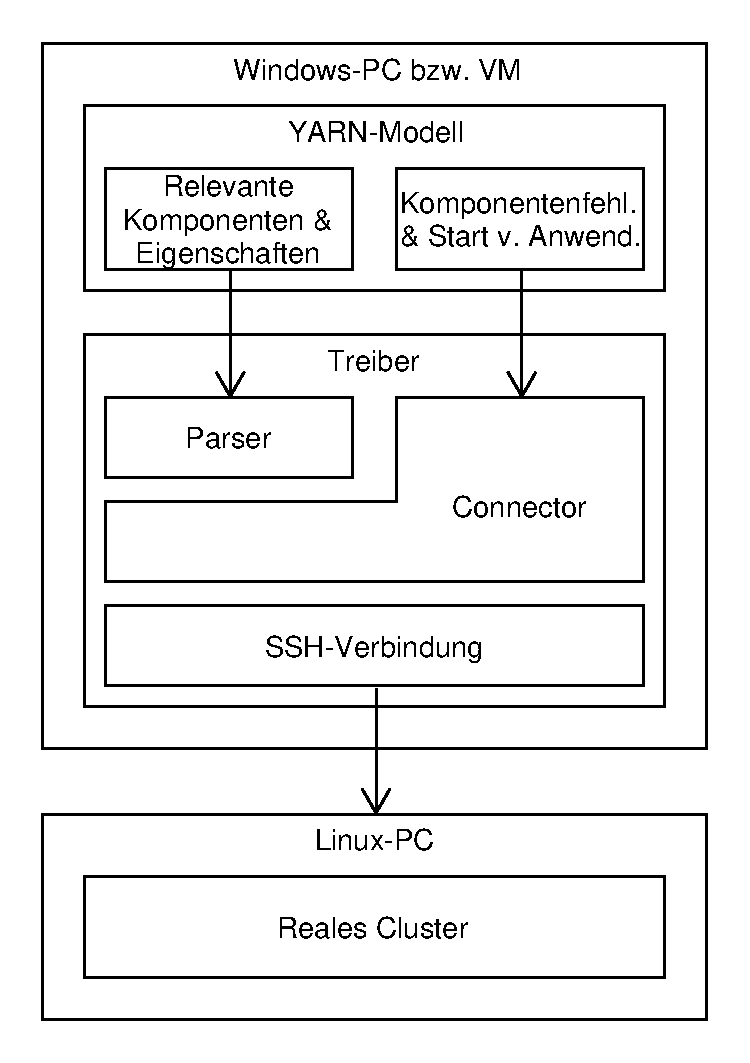
\includegraphics[width=0.5\columnwidth]
    {./images/modelArchitecture.pdf}
    \caption{Grundlegende Architektur des Gesamtmodells}
    \label{fig:modelArchitecture}
\end{wrapfigure}

Um Hadoop mit der Selfbalancing"=Komponente mit den in \autoref{sec:predictions} beschriebenen Behauptungen prüfen zu können, wird mithilfe des \ac{ss}"=Frameworks ein vereinfachtes Modell entwickelt.

Die rechts abgebildete \autoref{fig:modelArchitecture} beschreibt die grundlegende Architektur des Modells für diese Fallstudie.
Die Fallstudie besteht aus den drei Schichten des YARN"=Modells selbst, dem Treiber zum Herstellen der Verbindung zwischen dem Modell und dem realen Cluster sowie dem realen Cluster selbst.

Das eigentliche YARN"=Modell bildet die grundlegende Architektur von YARN bzw. YARN"=Anwendungen stark vereinfacht ab.
Es enthält daher nur die für diese Fallstudie relevanten Komponenten und Eigenschaften sowie die Definitionen der Komponentenfehler.

Die Verbindung zwischen dem Modell und dem realem Cluster bildet der Treiber als eigenständige Schicht.
Der Treiber besteht aus folgenden Komponenten:

\begin{description}
    \item [Parser] \hfill \\
        Verarbeitet die Monitoring"=Ausgaben vom realen Cluster und konvertiert diese für die Nutzung im YARN"=Modell.
    \item [Connector] \hfill \\
        Abstrahiert die Verbindung zum realen Cluster und die dabei auszuführenden Befehle.
    \item [SSH"=Verbindung]  \hfill \\
        Stellt die Verbindung zum realen Cluster her.
\end{description}

Der Zugriff mithilfe des Treibers auf das reale Cluster im Rahmen des Monitoring wird mithilfe des Parsers durchgeführt, welcher wiederum den Connector nutzt.
Bei anderen Zugriffen wie \zB die Injizierung und das Reparieren von Komponentenfehlern oder dem Starten von Anwendungen wird vom YARN"=Modell mithilfe des Connectors auf das reale Cluster zugegriffen.

Die Umsetzung des realen Clusters wird im folgenden \autoref{sec:aufbauCluster} beschrieben.
Die Umsetzung des YARN"=Modells und des Treibers wird im folgenden \autoref{chap:modell} beschrieben.


\section{Umsetzung des realen Clusters}\label{sec:aufbauCluster}

\citeauthor{zhang2016} haben im Rahmen ihrer gesamten Forschungsarbeit die Open"=Source"=Plattform Hadoop-Benchmark entwickelt und auf Github zur Verfügung gestellt.\footnote{\url{https://github.com/Spirals-Team/hadoop-benchmark}} Sie wurde speziell zum Einsatz in der Forschung erstellt und kann jederzeit an die eigenen Bedürfnisse angepasst werden. Zur Umsetzung des realen Clusters im Rahmen dieser Masterarbeit wurde daher eine speziell angepasste Version der Plattform eingesetzt.

\subsection{Plattform Hadoop-Benchmark}\label{sec:hadoopBenchmark}

Die Plattform ist in mehrere Szenarien unterteilt, darunter ein Hadoop in der Version 2.7.1 ohne Änderungen und ein darauf basierendes Szenario mit der Selfbalancing-Komponente. Hadoop-Benchmark basiert auf der Software \emph{Docker}\footnote{\url{https://www.docker.com/}} und dem dazugehörigen Tool \emph{Docker Machine}, um damit einfach und schnell ein Hadoop-Cluster aufbauen zu können. Mit \emph{Graphite}\footnote{\url{https://graphiteapp.org/}} ist zudem ein Monitoring-Tool enthalten, mit dem die Performance des Clusters überwacht und analysiert werden kann.

\begin{figure}
    \centering
    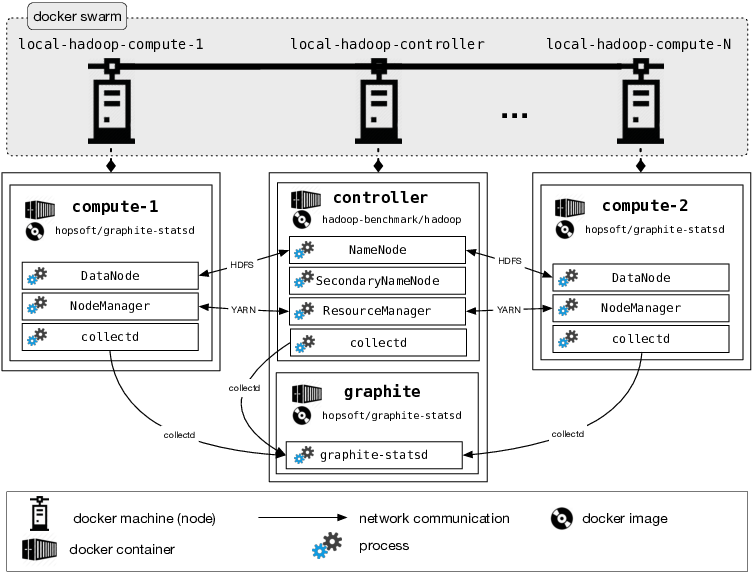
\includegraphics[width=.8\columnwidth]{./images/hadoopBenchmarkArch.png}
    \caption[High-Level-Architektur von Hadoop-Benchmark]{High-Level-Architektur von Hadoop-Benchmark \cite{abb:hadoopBenchmarkArch}}
    \label{fig:hadoopBenchmarkArchitecture}
\end{figure}

\autoref{fig:hadoopBenchmarkArchitecture} zeigt die grundlegende Architektur der Plattform, die mithilfe eines Docker-Swarms auf mehreren \emph{Docker Machines} (für den Einsatz von Docker eingerichtete virtuelle Maschinen) ein Cluster erstellt, auf denen dann in den Docker-Containern das eigentliche Hadoop-Cluster ausgeführt wird. Jeder Hadoop-Container enthält zudem das Tool \emph{collectd}\footnote{\url{https://collectd.org/}}, was das Monitoring des Containers auf Systemebene übernimmt und die Daten an den Graphite-Container auf der Controller-Machine übermittelt. Es ist dabei möglich, eine beliebige Anzahl an Nodes zu nutzen. Auch ist es möglich, den Docker Machines einen beliebig großen Arbeitsspeicher zur Verfügung zu stellen.

Die Plattform Hadoop-Benchmark enthält zudem einige Benchmark-Anwendungen:

\begin{itemize}[noitemsep]
    \item Hadoop Mapreduce Examples
    \item Intel HiBench\footnote{\url{https://github.com/intel-hadoop/HiBench}}
    \item SWIM (Statistical Workload Injector for Mapreduce)\footnote{\url{https://github.com/SWIMProjectUCB/SWIM}}
\end{itemize}

Eine Besonderheit bildet der SWIM-Benchmark, welcher sehr Ressourcenintensiv ist und daher auf einem \emph{Single Node Cluster}, also einem kompletten Hadoop-Cluster auf nur einem Computer, sehr zeitintensiv sein kann. Der Intel HiBench-Benchmark besteht aus Kategorien wie \emph{Machine Learning} oder Graphen, welche wiederum aus einen oder mehreren \emph{Workloads} bestehen, welche entsprechende Anwendungen bzw. Algorithmen auf dem Hadoop-Cluster ausführen. Einige der Hibench-Workloads basieren auf den Mapreduce Examples, welche wiederum voneinander unabhängige Beispielanwendungen für Hadoop darstellen.

\subsection{Anpassungen und Setup}\label{sec:clusterFallstudie}

Da mithilfe der Plattform Hadoop-Benchmark die Erstellung eines Hadoop-Clusters massiv vereinfacht wird, kommt die Plattform auch in dieser Masterarbeit zum Einsatz. Da Docker und Hadoop aber vor allem für den Einsatz in einer Linux-Umgebung entwickelt wurden, wird dazu ein eigener PC mit Ubuntu 16.04 LTS genutzt. Da \sS das .NET-Framework, und damit Windows, benötigt, wird dafür ebenfalls ein eigener PC verwendet. Im konkreten Versuchsaufbau wird für Windows eine VM genutzt, welche auf einem anderen PC als das Cluster ausgeführt wird. Die genauen Spezifikationen der PCs und der Windows-VM sind in \autoref{tab:pcSpecs} aufgelistet. Die Windows-VM und der Cluster-PC werden mithilfe von SSH-Verbindungen miteinander verbunden.

\begin{table}
    \centering
    \begin{tabular}{|c|c|c|c|}
    	\hline
    	 \textbf{}   & \textbf{Cluster-PC} &         \textbf{VM-PC}          & \textbf{Windows-VM}  \\ \hline\hline
    	\textbf{CPU} & \multicolumn{2}{c|}{Intel Core i5-4570 @ 3,2 GHz x 4} &     4 CPU Cores      \\ \hline
    	\textbf{RAM} &              \multicolumn{2}{c|}{16 GB}               &         8 GB         \\ \hline
    	\textbf{SSD} &       512 GB        &             512 GB              &  $\leq$ 100 GB VHD   \\ \hline
    	\textbf{OS}  &  Ubuntu 16.04 LTS   &        Ubuntu 16.04 LTS         & Windows 10 1709 Edu. \\ \hline
    \end{tabular}
    \caption{Spezifikationen der verwendeten PCs und Windows-VM}
    \label{tab:pcSpecs}
\end{table}

Auf dem Cluster-PC nutzt Docker-Machine zur Erstellung, Verwaltung und Ausführung der VMs die Treiber von VirtualBox 5.2\footnote{\url{https://www.virtualbox.org/}}, zum Abrufen der Daten der REST-API über die SSH-Verbindung wird \emph{curl}\footnote{\url{https://curl.haxx.se/}} genutzt. Für das Cluster werden 4 Nodes, der Controller sowie eine Consul-VM zur internen Verwaltung der Netzwerkverbindungen zwischen den VMs und Docker-Containern erstellt. Der Controller erhält 4 GB RAM, jeder der vier Nodes jeweils 2 GB, für den Consul sind 512 MB ausreichend. Für die Windows-VM wird ebenfalls VirtualBox 5.2 eingesetzt.

%TODO: Link zum angepassten Hadoop-Benchmark?
In keinem Szenario der Plattform Hadoop-Benchmark wird standardmäßig der \ac{TLS} von Hadoop gestartet. Daher wurde für diese Fallstudie basierend auf dem Selfbalancing-Szenario ein neues Szenario erstellt, bei dem der \ac{TLS} gestartet wird. Dadurch ist einerseits die Selfbalancing-Komponente von \citeauthor{zhang2016} aktiv und andererseits besteht die Möglichkeit, für das Monitoring zusätzlich den \ac{TLS} zu nutzen.

Um viele standardmäßige Aufgaben und Möglichkeiten zu vereinfachen, wurde zudem ein eigenes Setup-Script erstellt. Es vereinfacht folgende Aufgaben:

\begin{itemize}[noitemsep]
    \item Starten, Beenden und Löschen des kompletten Clusters mit Hadoop
    \item Starten und Beenden des Docker-Containers eines Nodes
    \item Hinzufügen und Entfernen der Netzwerkverbindung des Docker-Containers eines Nodes
    \item Ausführen der verwendeten Benchmarks
    \item Ausführen von eigenen Befehlen auf dem Docker-Container des Controllers
\end{itemize}

Für die Befehle, die das gesamte Cluster betreffen, wird vom Setup-Script meist auf das in Hadoop-Benchmark enthaltene Start-Script zugegriffen. Die Befehle, welche die Docker-Container der Nodes betreffen, sowie das Ausführen von Befehlen im Controller-Container, werden vom Setup-Script direkt ausgeführt. Für das Starten der Benchmarks werden dagegen die in Hadoop-Benchmark enthaltenen Ausführungs-Scripte der Benchmarks gestartet.
